\section{January 2021}
%------------------------------------------------------------
\begin{mathbox}{\text{\subsection{A Simple Proof}}}
{Are there infinitely many prime numbers? If yes, how do we prove they exist?\\
Here's a simple proof.\\
{Assume} we have only $n$ prime numbers; $P_1, P_2, P_3, \dots P_n$.
\begin{align*}
\text{Let}~N = P_1 \cdot P_2 \cdot P_3 \dots P_n + 1
\end{align*}
$N$ {isn't divisible} by any of the primes $P_1, P_2, P_3, \dots P_n$\footnote{Prime numbers start from $2$ and $N$ is the LCM of all the prime numbers added to $1$.}  which implies $N$'s {prime factorisation} is $N \times 1$. $N$ being prime {contradicts} our initial assumption.\\
Thus, there exist infinite primes. QED}
\end{mathbox}
%------------------------------------------------------------
\begin{phybox}{\text{\subsection{Neutrons and Protons have Components too!}}}
{Have you ever wondered whether {protons, neutrons and electrons; the constituents of an atom,} can be {divided further} into constituting components? The answer is {"Yes"}. A {quark} is an elementary particle and a fundamental constituent of matter. Quarks combine to form particles called hadrons. All commonly observable matter is composed of {up quarks, down quarks and electrons}. Quarks are never found existing individually, they can be found only composing {hadrons}, which include {baryons} (protons and neutrons) and {mesons}, or in {quark–gluon plasma}.}
\end{phybox}
%------------------------------------------------------------
\begin{chembox}{\text{\subsection{A Salty Bond}}}
{The {Ionic bond} is a type of a {chemical bond} that is a result of the attraction {between oppositely charged particles} in ionic compounds like NaCl\footnote{More examples; KCl, CaCl_2}. Ions are atoms (or a group of atoms) having a {net charge}. Atoms that {gain electrons} to become {stable} are called {anions} while those that {lose electrons} for the same are called {cations}. This {transfer of electrons} is known as {electrovalence}. Ionic bonds are {mostly} formed {between metals and non-metals}. In simpler words, an ionic bond is a result of the transfer of electrons from a metal (cation) to a non-metal (anion) in order for both atoms to attain stability.}
\end{chembox}
%------------------------------------------------------------
\begin{mathbox}{\text{\subsection{Exponentiation^{-1}}}}
{The {logarithm} function (denoted by $\log$) is the {inverse} function of {exponentiation}. It denotes the {exponent/power} to which the {'base'} has been raised to in a number. Here's an example;
\begin{align*}
    \text{Let } x = a^b. \text{ This implies} \log_a (x) = b
\end{align*}
The logarithm of $x$ to the base $a$ can be a {whole number, decimal number, irrational number} or even a {complex number} depending on its value. Often, log graph are used to make growth, forecast and even the number of cases during a pandemic. Logarithms involving complex numbers\footnote{\sffamily${\sqrt{-x}, \sqrt[3]{-x}, \dots}$} $(i)$ can be plotted on the real-complex plane.}
\end{mathbox}
%------------------------------------------------------------
\begin{phybox}{\text{\subsection{Heisenberg's Life Questioning Inequality}}}
{In quantum mechanics\footnote{Branch of Physics dedicated to observing the physical properties at the subatomic scale.}, the uncertainty principle (also known as Heisenberg's uncertainty principle) is a variety of mathematical inequalities asserting a fundamental limit to the accuracy with which the values for certain pairs of physical quantities of a particle, such as position ($x$) and momentum ($p$) can be predicted from initial or known conditions. Heisenberg, in simple words stated that if you know velocity/momentum of the particle, you can't find it's position and vice versa. The equation stated in favour;
\begin{align*}
    \Delta x \times \Delta P \geq \frac{h}{4\pi}
\end{align*}
where  $h = 6.626 \times 10^-34$ (Planck's Constant).\\
The more precisely the position of some particle is determined, the less precisely its momentum/velocity can be predicted from the known initial conditions.}
\end{phybox}
%------------------------------------------------------------
\begin{mathbox}{\text{\subsection{{Prime Number Theorem}}}}
{The prime number theorem describes the asymptotic\footnote{Asymptotic here means approximate in mathematical terms.} distribution of prime numbers among positive integers. It formalizes the intuitive idea that primes become less common as they become larger. The prime number theorem addresses this by precisely quantifying the rate at their frequency decreases. The first breakthrough was the $\pi(n)$ function, which calculates the probability that a random integer less than or equal to $n$ is prime. It's defined as;
\begin{align*}
    \pi(n) \sim \frac{1}{\ln(n)}
\end{align*}
where $\ln (n)$ is the natural logarithm\footnote{$\log_e(n)$} of $n$.}
\end{mathbox}
%------------------------------------------------------------
\begin{mathbox}{\text{\subsection{Catalan's Conjecture}}}
{The Catalan's conjecture, conjectured by the mathematician Eugène Charles Catalan in 1844 and proven in 2002 by Preda Mihăilescu. It states that there  exists only one solution to the equation
\begin{align*} 
    x^a - y^b = 1
\end{align*} 
where $x=3, a=2, y=2, b=3$ for {$a,b > 1$} and {$x,y > 0$}.}
\end{mathbox}
%------------------------------------------------------------
\begin{phybox}{\text{\subsection{Angular Momentum of an Electron}}}
{The {angular momentum} $(L)$ of an {electron} in the $n^{th}$ orbit is given by 
\begin{align*} 
    L = \frac{nh}{2\pi} 
\end{align*} where $h$ is the {Planck's constant}.}
\end{phybox}
%------------------------------------------------------------
\begin{chembox}{\text{\subsection{Gibbs Free Energy}}}
{In thermodynamics, the {Gibbs Free Energy} $(G)$ (named after Josiah Willard Gibbs) is a {thermodynamic potential} that calculates the {maximum reversible work} performed by a thermodynamic system at a {constant temperature} $(T)$ and pressure{} $(P)$. It is given by 
\begin{align*} 
    \Delta G=\Delta H-T\Delta S 
\end{align*} where $S$ represents its {Entropy}, i.e. the measure of randomness. {S.I unit - Joules}}
\end{chembox}
%------------------------------------------------------------

\begin{chembox}{\text{\subsection{Quantum Numbers (Not a new System!?)}}}
{In chemistry and quantum physics, quantum numbers describe values of conserved quantities in the dynamics of a quantum system. 
An important aspect of quantum mechanics is the quantization of many observable quantities of interest. In particular, this leads to quantum numbers that take values in discrete sets of integers or half-integers\footnote{Numbers of the form $\frac{2n+1}{2}$}; although they approach infinity in some cases. Quantum numbers often describe specifically the energy levels of electrons in atoms, but other possibilities include angular momentum, spin, etc. An important family is flavour quantum numbers – internal quantum numbers which determine the type of a particle and its interactions with other particles through the fundamental forces. A system can have one or more quantum numbers; it is thus difficult to list all possible quantum numbers.\\
Four quantum numbers can describe an electron in an atom completely:
\begin{itemize}
    \item{Principal quantum number $(n)$}
    \item{Azimuthal quantum number $(l)$}
    \item{Magnetic quantum number $(m)$}
    \item{Spin quantum number $(s)$}
\end{itemize}}
\end{chembox}
%------------------------------------------------------------
\begin{chembox}{\text{\subsection{Principal Quantum Number}}}
{In quantum mechanics, the principal quantum number (symbolized by $n$) is one of four quantum numbers assigned to each electron in an atom to describe that electron's state. Its values are natural numbers making it a discrete variable.\\
Apart from the principal quantum number, the other quantum numbers for bound electrons are the azimuthal quantum number $l$, the magnetic quantum number $m$, and the spin quantum number $s$.
As $n$ increases, the electron also has higher energy and is, therefore, less tightly bound to the nucleus. For higher $n$ the electron is farther from the nucleus. For each value of $n$ there are $n$ accepted $l$ (azimuthal) values ranging from $0$ to $n − 1$ inclusively, hence higher-$n$ electron states are numerous in definition. Accounting for two states of spin, each $n$-shell can accommodate up to $2n^2$ electrons (Given by Niels Bohr).\\
The principal quantum number was first created for use in the semi-classical Bohr model of the atom, distinguishing between different energy levels. With the development of modern quantum mechanics, the simple Bohr model was replaced with a more complex theory of atomic orbitals. However, the modern theory still requires the principal quantum number.}
\end{chembox}
%------------------------------------------------------------
\begin{chembox}{\text{\subsection{Azimuthal Quantum Number}}}
{The azimuthal quantum number is a quantum number for an atomic orbital that determines its orbital angular momentum as well as the shape of the orbital. The azimuthal quantum number is the second set of quantum numbers which describes the unique state of an electron (the others being the principal quantum number, the magnetic quantum number, and the spin quantum number). It is also known as the orbital angular momentum quantum number, orbital quantum number or second quantum number, and is symbolized as $l$.\\
Each of the different angular momentum states can take $2(2l + 1)$ electrons. This is because the third quantum number $m$ (which can be thought of loosely as the quantized\footnote{Restricting the number of possible values of a quantity or states of a system so that certain variables can assume only certain magnitudes.} projection of the angular momentum on the z-axis) runs from $−l$ to $l$ in integer units, and so there are $2l + 1$ possible states. Each distinct $n, l, m$ orbital can be occupied by two electrons with opposing spins (given by the quantum number $s = \pm \frac{1}{2}$), giving $2(2l + 1)$ electrons overall. Orbitals with higher $l$ than given in the table are perfectly permissible, but these values cover all atoms so far discovered.}
\end{chembox}
%------------------------------------------------------------
\begin{chembox}{\text{\subsection{Magnetic Quantum Number}}}
{The magnetic quantum number (symbol $m_l$) is one of four quantum numbers in atomic physics. The set is: principal quantum number, azimuthal quantum number, magnetic quantum number, and spin quantum number. Together, they describe the unique quantum state of an electron. The magnetic quantum number distinguishes the orbitals available within a subshell, and is used to calculate the azimuthal component of the orientation of orbital in space. Electrons in a particular subshell (such as $s, p, d, $or$ f$) are defined by values of $l (0, 1, 2, or 3)$. The value of $m$ can range from $-l$ to $+l$, including zero. Thus the $s, p, d, $and$ f$ subshells contain $1, 3, 5, and 7$ orbitals each, with values of $m$ within the ranges $0, \pm 1, \pm 2, \pm 3$ respectively. Each of these orbitals can accommodate up to two electrons (with opposite spins), forming the basis of the periodic table.}
\end{chembox}
%-----------------------------------------------------------------
\begin{chembox}{\text{\subsection{Spin Quantum Number}}}
{In atomic physics, the spin quantum number is a quantum number that describes the intrinsic angular momentum (or spin angular momentum, or simply spin) of a given particle. The spin quantum number is designated by the letter $s$, and is the fourth of a set of quantum numbers (the principal quantum number, the azimuthal quantum number, the magnetic quantum number, and the spin quantum number), which completely describe the quantum state of an electron.
this can be written as:-
\begin{align*}
 ||s|| = \sqrt{s(s+1)}h
\end{align*}
where, 
\begin{itemize}
    \item {$s$ is the spin vector }
    \item{$||s||$ is the norm of spin vector}
    \item{$h$ is the Planck constant}
\end{itemize}
}
\end{chembox}
%-----------------------------------------------------------------
\begin{mathbox}{\text{\subsection{Modular Arithmetic and Weird Prime Pairs}}}
{Modular Arithmetic is an operation (used extensively in Mathematical Olympiads and Number Theory) to compute the remainder when a number is divided by another. For example, say $5$ is the remainder when $a$ is divided by $b$. We can represent it the following way:
\begin{align*}
    a \equiv 5 \pmod b
\end{align*}
where $\pmod b$ represents $a$ taken modulo $b$ and $5$ is $a \pmod 5$.}\\
Modulos can also be thought of this way. We know that $14 \equiv 2 \pmod 3$. On adding $3$ to the remainder, we get $14 \equiv 5 \pmod 3$. But this is true too (since $14$ leaves a remainder of 5 on being divided by $9$). Are we arriving upon a paradox? No, not at all.
This actually leads us to our next point.\\
A property of congruence systems is that;\\
if $a \equiv b \pmod n$ it implies $(\implies)~a \equiv b + n \pmod n$.\\
Modular Arithmetic systems also have the following properties;
\begin{itemize}
    \item{If $a \equiv b \pmod n$ and $c \equiv d \pmod n;~ab \equiv cd \pmod n$}
    \item{If $a \equiv b \pmod n$ and $c \equiv d \pmod n;~a + b \equiv c + d \pmod n$}
\end{itemize}
The same apply for subtraction and division respectively.
\end{mathbox}
%-----------------------------------------------------------------
\begin{mathbox}{\text{\subsection{Quadratic Residues (Actually not Residual!)}}}
{An interesting part of modular arithmetic congruence systems is quadratic residues which represent the remainder when a perfect square is divided by some integer $n$. \\
For example, one can observe that $0$ and $1$ are the quadratic residues when any perfect square is taken modulo $4$; i.e.$\pmod 4$.\\
This has a very simple proof. We know that any integer $x$ is either $0, 1, 2$ or $3 \pmod 4$. From the multiplicative property,
\begin{center}
    $x \equiv 0, 1, 2, 3 \pmod 4\\
    \implies x \times x \equiv 0 \times 0, 1 \times 1, 2 \times 2, 3 \times 3 \pmod 4\\
    \implies x \equiv 0, 1, 4, 9 \pmod 4\\
    \text{On writing $4$ and $9$ as $4 + 0$ and $2\times 4 + 1$},\\
    $x$ \equiv 0, 1 \pmod 4$
\end{center}
The following table lists quadratic residues when taken$\pmod n$}
\begin{center}
\begin{tabular}{ |c|c| } 
    \hline
    $n$ & $x^2 \pmod n$\\
    \hline
    $1$ & $0$\\
    $2$ & $0, 1$\\
    $3$ & $0, 1$\\
    $4$ & $0, 1$\\
    $5$ & $0, 1, 4$\\
    $6$ & $0, 1, 3, 4$\\
    $7$ & $0, 1, 2, 4$\\
    $8$ & $0, 1, 4$\\
    \hline
\end{tabular}
\end{center}
\end{mathbox}
%-----------------------------------------------------------------
\begin{mathbox}{\text{\subsection{Pell's Equation}}}
{Pell's equation, also called the Pell–Fermat equation, is any Diophantine equation of the form 
\begin{align*}
x^{2}-ny^{2}=1
\end{align*}
where $n$ is a given positive non-square integer. It has infinitely many solutions (proved by Joseph Lagrange) in $x$ and $y$ and forms a hyperbola when plotted in Cartesian co-ordinates.\\
We can also find its solutions through a recursive algorithm where;\\
If $(x_{0},y_{0})$ is a solution to $x^{2}-dy^{2}=N$ and $(u_{n},v_{n})$ is a solution to $u^{2}-dv^{2}=1$ then $(x_n,y_n)$ such that $x_n+y_n \sqrt{d}=(x_{0}+y_{0}{\sqrt{d}})$ is a solution to $x^{2}-dy^{2}=N.$\\
This is the graph for $n = 2$:\\
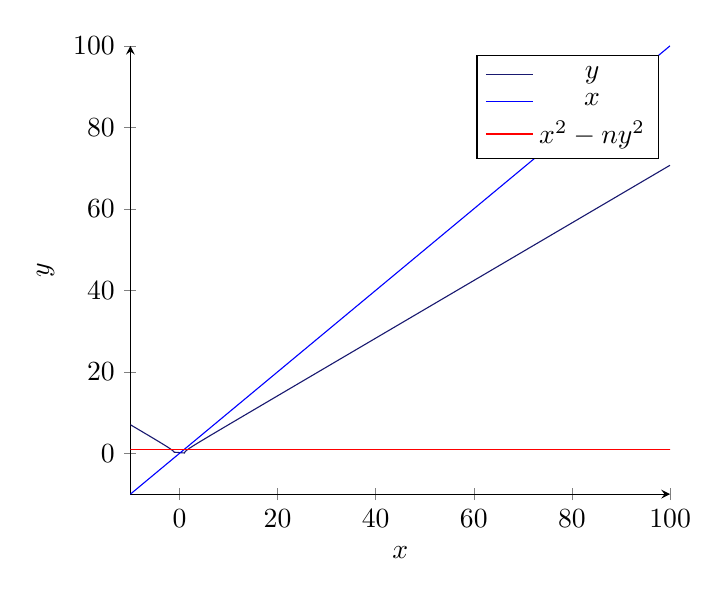
\begin{tikzpicture}
\begin{axis}[
    axis lines = left,
    xlabel = $x$,
    ylabel = {$y$},
]
\addplot [
    domain=-10:100, 
    samples=1000, 
    color=MidnightBlue,
]
{((x^2 - 1)/2)^0.5};
\addlegendentry{$y$}
\addplot [
    domain=-10:100, 
    samples=1000, 
    color=blue,
]
{x};
\addlegendentry{$x$}
\addplot [
    domain=-10:100, 
    samples=1000, 
    color=red,
]
{1};
\addlegendentry{$x^2 - ny^2$}
\end{axis}
\end{tikzpicture}}
\end{mathbox}
%------------------------------------------------------------
\begin{phybox}{\text{\subsection{Pauli's "Excluded" Principle}}}
{The Pauli's exclusion principle is the quantum mechanical principle which states that two or more identical fermions\footnote{Particles with half-integer spin} cannot occupy the same quantum state within a quantum system simultaneously. This principle was formulated by Austrian physicist Wolfgang Pauli in 1925 for electrons, and later extended to all fermions with his spin–statistics theorem of 1940.
In the case of electrons in atoms, it can be stated as follows: it is impossible for two electrons of a poly-electron atom to have the same values of the four quantum numbers: $n$, the principal quantum number, $l$, the azimuthal quantum number, $m$, the magnetic quantum number, and $s$, the spin quantum number. For example, if two electrons reside in the same orbital, then their $n$, $l$, and $m$ values are the same, therefore their $s$ must be different, and thus the electrons must have opposite half-integer spin projections of $\frac{1}{2}$ and $-\frac{1}{2}$.}
\end{phybox}
%-------------------------------------------------------------
\begin{phybox}{\text{\subsection{Half life Of Atoms}}}
{Half-life represented by $t_\frac{1}{2}$ is the time required for a quantity to reduce to half of its initial value. It’s used in nuclear physics to describe how quickly unstable atoms undergo radioactive decay or how long stable atoms survive. Half-life is mainly defined in terms of probability; i.e. ”Half-life is the time required for exactly half of the entities to decay on average”. In other words, the probability of a radioactive atom decaying within its half-life is 50%.\\
Exponential decay can be described by any of the following three equivalent formulas:
\begin{align*}
N(t)=N_{0}\left({\frac{1}{2}}\right)^{\frac{t}{t_{1/2}}}\\
N(t)=N_{0}e^{-{\frac {t}{\tau }}}\\
N(t)=N_{0}e^{-\lambda t}
\end{align*}
where;
\begin{itemize}
\item{$N_0$ is the initial quantity of the substance that will decay,}
\item{$N(t)$ is the quantity that still remains and has not yet decayed after a time $t$,}
\item{$t_\frac{1}{2}$ is the half-life of the decaying quantity, $\tau$ is a positive number called the mean lifetime of the decaying quantity,}
\item{$\lambda$ is a positive number called the decay constant of the decaying quantity.}
\end{itemize}
The three parameters $t_\frac{1}{2}$, $\tau$, and $\lambda$ are all directly related in the following way:
\begin{align*}
t_\frac{1}{2}={\frac {\ln(2)}{\lambda }}=\tau \ln(2)
\end{align*}}
\end{phybox} 
%------------------------------------------------------------
